
\begin{figure*}[t]
\centering
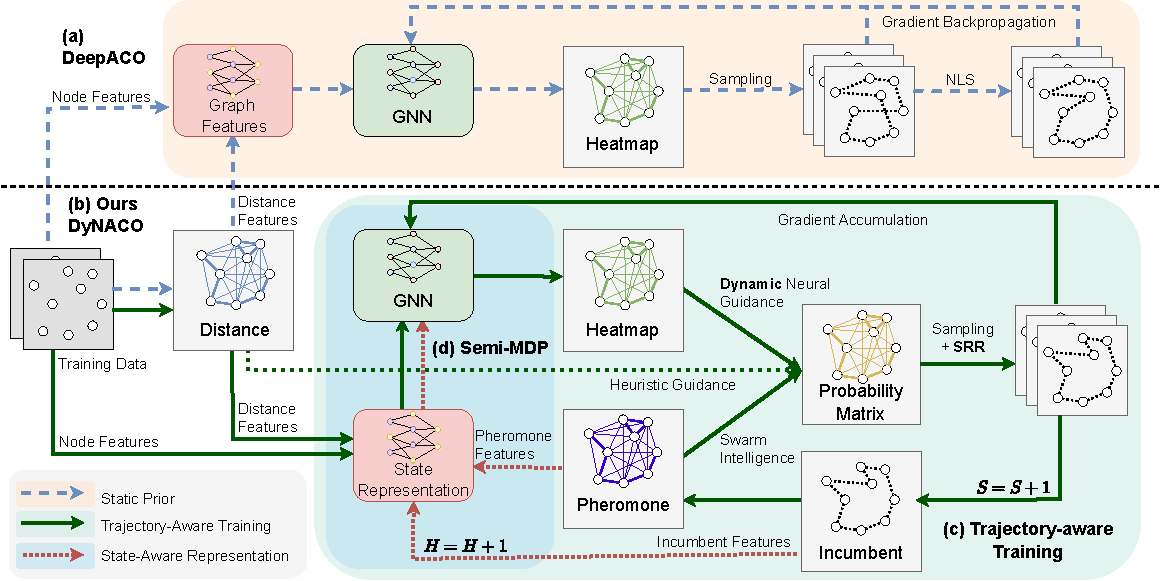
\includegraphics[width=\textwidth]{figures/overview.pdf}
\caption{\emph{Comparison of training paradigms and our \DyNACO{}.} (a) The original DeepACO paradigm~\cite{deepaco, gfacs, gtgaco}. (b) Our \DyNACO{} framework for dynamic guidance. (c) Trajectory-aware training that aligns with iterative search dynamics. (d) State-aware representation conditioning the policy on the evolving search state.}
\label{fig:guidance-loop}
\end{figure*}

% Standard ACO constructs solutions using transition probabilities $p(j \mid i) \propto [\tau_{ij}]^\alpha [\eta_{ij}]^\beta$, relying on an evolving pheromone matrix $\tau_{ij}$ but a strictly static heuristic visibility $\eta_{ij}$. 
% Based on the notation introduced in Section~\ref{sec:prelim}, we present \DyNACO{}, a dynamic neural-guided ACO framework that periodically observes the evolving search state and emits trajectory-aware edge guidance for the next block of ACO iterations.
% This section presents \DyNACO{}, 
Based on the notation introduced in Section~\ref{sec:prelim}, we present the method in the same progression used by the search system itself. We first define \DyNACO{}, Dynamic Neural Ant Colony Optimization: one state-aware policy repeatedly observes the evolving ACO state and emits guidance over the full search trajectory rather than committing to a one-shot heatmap. We then build \DyNACS{}, Dynamic Neural Ant Colony Search, on top of this base model by giving different ant groups complementary trajectory distributions within a shared colony. Finally, we describe the scalable search environment shared by both models: a perturbation-based ACO backend with scope-restricted refinement that makes the conceptual policy interface trainable and scalable. We instantiate the framework for Euclidean \TSP{} on $N$ nodes, seeking a tour $\pi$ that minimizes total cost $C(\pi)$, and for \CVRP{}, where we use a capacity-aware perturbation backend for feasibility handling.

\subsection{Semi-MDP Formulation}
\label{sec:mdp}
Prior neural-guided ACO methods~\cite{deepaco,gfacs,gtgaco} treat guidance as a \emph{one-shot prediction}: a network observes the instance graph and emits a static heatmap, trained from a single pheromone-free sample of ants, after which the solver runs a full ACO loop with pheromone dynamics to completion without further interaction. The model is therefore trained without pheromone dynamics. We address this mismatch by formalizing \DyNACO{} as a two-level hierarchy in which a neural \emph{meta-policy} $\pi_\theta$ repeatedly observes the macro-state and emits updated guidance, while the ACO backend executes $S$ iterations between observations. The policy follows the evolving ACO state rather than a fixed inference horizon, so it can be evaluated under longer ACO budgets by continuing to observe the current macro-state. Such a semi-MDP formulation enables:

\begin{enumerate}
\item \emph{Amortized policy updates.} The neural policy outputs actions only once every $S$ iterations and remains fixed during this interval. This amortizes overhead and effectively reduces variance during policy-gradient training.
\item \emph{Efficient PPO replay.} By framing the guidance process as a semi-MDP, we avoid tracking low-level internal ACO ant steps. To compute PPO importance ratios for off-policy reinforcement learning updates, we only need to store the macro-states at the update steps: the pheromone snapshots, incumbent features, and action traces.
\item \emph{Trajectory-aware objective.} Instead of a myopic single-step reward as used in the literature, we minimize the long-term cumulative cost $\sum_{h=1}^H C_h$ across the full MDP trajectory.
\end{enumerate}

Formally, we model this as a \emph{semi-MDP with fixed-duration macro-actions} as follows:
\begin{itemize}[topsep=0pt]
\item \emph{State} $\mathcal{S}_h = (G, \tau^{(h,0)}, b^{(h)})$: At update step $h$, the macro-state comprises the static $K$-nearest-neighbor candidate graph $G$, the pheromone matrix $\tau^{(h,0)} \in \mathbb{R}^{N \times K}$ at the start of the interval (indexed as $h,0$), and the current solution $b^{(h)}$.
\item \emph{Action} $a_h = z_\theta(\mathcal{S}_h) \in \mathbb{R}^{N \times K}$: A residual logit matrix emitted by the \DyNACO{} policy that shapes the pheromone matrix.
\item \emph{Transition} $P(\mathcal{S}_{h+1} \mid \mathcal{S}_h, a_h)$: The environment executes $S$ internal iterations of ACO (comprising ant sampling, scope-restricted refinement, and pheromone updates), functioning as a stochastic, state-dependent transition kernel.
\item \emph{Cost} $C_h = \frac{1}{S \cdot m} \sum_{s=1}^{S} \sum_{a=1}^{m} C(\hat{\pi}_{a,s})$: The average post-refinement tour cost across all $m$ ants over the $S$ iterations. Our objective is to minimize the expected cumulative cost $\sum_{h=1}^H C_h$.
\end{itemize}

% ======================================================================
% 3.3 State-Aware Policy and Training
% ======================================================================
\subsection{State-Aware Policy and Trajectory-Aware Training}
\label{sec:agent}


\smallskip\noindent\textbf{State-Aware Representation.}
\label{sec:state}
Prior neural-ACO methods condition solely on \emph{static} instance geometry, yielding guidance that cannot adapt to the solver's evolving state. The semi-MDP state $\mathcal{S}_h = (G,\, \tau^{(h,0)},\, b^{(h)})$ defined in Section~\ref{sec:mdp} isolates the two quantities that evolve between guidance updates: the pheromone field~$\tau$ and the incumbent solution~$b$. These are precisely the signals inherent to the ACO process; conditioning on them enables the semi-MDP formulation and renders the guidance \emph{dynamic}. We retain the static node features used by DeepACO~\cite{deepaco} for each problem and add three sparse edge channels on the $K$-NN graph: scale-normalized distance, local pheromone concentration, and an incumbent-edge indicator. The dynamic channels are recomputed at every outer step, remain bounded by $\mathcal{O}(N \cdot K)$, and are processed by a 12-layer GNN encoder~\cite{deepaco} with interleaved node and edge message passing. Appendix~\ref{app:features} gives the exact feature definitions.

The \DyNACO{} policy outputs a scalar guidance score $z_{ij}$ for each candidate edge via a 3-layer MLP decoder.
The shaped transition kernel adds these logits in log-space (Eq.~\ref{eq:held-logits}), corresponding to a KL-regularized policy where $p^\theta(\cdot\mid i) \propto q(j\mid i)\exp(z_{ij})$.
Because $\tau_{\min} > 0$ and logits remain finite, every candidate retains positive probability; the policy redistributes mass but cannot exclude edges.
\begin{algorithm}[t]
\caption{PPO training for dynamic \DyNACO{}.}
\label{alg:train}
\begin{algorithmic}[1]
\REQUIRE $\theta$ (policy params), $E$ (epochs), $H$ (outer steps), $S$ (inner steps), $K_{\text{PPO}}$ (PPO epochs), $m$ (ants)
\FOR{$e = 1 \to E$}
    \STATE $x \sim \mathcal{X}$; \, $\tau^{(1,0)} \gets \tau_{\max}$; \, $b^{(1)} \gets \textsc{Greedy}(x)$
    \FOR{$h = 1 \to H$}
        \STATE $z \gets z_{\theta_{\text{old}}}(\mathcal{S}_h)$; \, $\mathcal{D}_h \gets \emptyset$
            \COMMENT{Outer: emit guidance}
        \FOR{$s = 1 \to S$}
            \STATE $\{\pi_{a,s}\}_{a=1}^m \gets \textsc{Sample}(p^\theta, \tau^{(h,s)}, z, b^{(h)})$
                \COMMENT{Inner: ACO sampling}
            \STATE $\mathcal{D}_h \gets \mathcal{D}_h \cup \{(\tau^{(h,s)}, \{\pi_{a,s}\}, \{C(\hat{\pi}_{a,s})\})\}$
            \STATE $a^* \gets \argmin_a C(\hat{\pi}_{a,s})$; \, $b^{(h)} \gets \min(b^{(h)}, \hat{\pi}_{a^*,s})$
            \STATE $\tau^{(h,s+1)} \gets (1{-}\rho)\tau^{(h,s)} + \rho \cdot \Delta\tau(b^{(h)})$
        \ENDFOR
        \STATE $\tau^{(h+1,0)} \gets \tau^{(h,S)}$; \, $b^{(h+1)} \gets b^{(h)}$
        \FOR{$k = 1 \to K_{\text{PPO}}$}
            \STATE $\theta \gets \theta - \nabla_\theta \mathcal{L}^{\text{PPO}}(\theta; \mathcal{D}_h, z_\theta(\mathcal{S}_h))$
                \COMMENT{PPO update}
        \ENDFOR
    \ENDFOR
\ENDFOR
\end{algorithmic}
\end{algorithm}



\smallskip\noindent\textbf{Trajectory-Aware Training.}
\label{sec:training}
Prior methods~\cite{deepaco,gfacs,gtgaco} optimize a \emph{single-step} objective: $\min_\theta \mathbb{E}_{\pi \sim p_\theta(\cdot \mid G)} [ C(\pi) ]$, where ants sample once from the neural heuristic alone.
At inference, however, the same static heatmap is inserted into a full ACO loop where pheromone fields evolve over hundreds of iterations.
This discrepancy precludes learning adaptive behavior: because training never exposes the model to pheromone dynamics, the heatmap inevitably conflicts with the pheromone landscape in later iterations.

We instead optimize the expected per-iteration post-SRR cost across the full trajectory.
Let $\hat{\pi}_{a,s} = \mathrm{LS}(\pi_{a,s})$ denote the tour produced by ant $a$ at sampling iteration $s$ after local search:
\begin{equation}
J(\theta) = \mathbb{E} \left[ \frac{1}{I} \sum_{h=1}^H \sum_{s=1}^S \frac{1}{m} \sum_{a=1}^m C(\hat{\pi}_{a,s}) \right].
\end{equation}
This \emph{trajectory-aware} objective averages cost over all $I = H \times S$ iterations, training the policy to remain effective from early exploration through late exploitation and minimizing the area under the cost curve rather than a single endpoint.

Under perturbative sampling each ant modifies at most $M$ edges, and the log-probability of its trajectory is the sum over stochastic edge choices.
Because the number of stochastic decisions $T_a$ varies across ants (deterministic steps with a single feasible candidate contribute $\log p = 0$), we normalize by decision count: $\bar{\ell}_{a,s} = \frac{1}{T_a} \sum_{t=1}^{T_a} \log p^\theta(v_t \mid u_t)$.
This per-decision normalization prevents ants with more stochastic steps from dominating the gradient.
We compute a per-iteration baseline $b_s = \frac{1}{m}\sum_{a=1}^{m} C(\hat{\pi}_{a,s})$ and define advantage as $A_{a,s} = b_s - C(\hat{\pi}_{a,s})$, so that better-than-average tours receive positive advantage.
For PPO we normalize advantages across the batch: $\hat{A}_{a,s} = (A_{a,s} - \mu_A) / (\sigma_A + \epsilon)$.

% \begin{table*}[t]
% \centering
% \caption{Comparative results on synthetic \TSP{} and \CVRP{} instances. OOM: out of memory.}
% \label{tab:main-results}
% \small
% \renewcommand{\arraystretch}{0.8}
% \resizebox{\textwidth}{!}{
% \begin{tabular}{lcccccccccc}
% \toprule
% & \multicolumn{2}{c}{\TSP{}1K} & \multicolumn{2}{c}{\TSP{}5K} & \multicolumn{2}{c}{\TSP{}10K} & \multicolumn{2}{c}{\TSP{}50K} & \multicolumn{2}{c}{\TSP{}100K} \\
% \cmidrule(lr){2-3} \cmidrule(lr){4-5} \cmidrule(lr){6-7} \cmidrule(lr){8-9} \cmidrule(lr){10-11}
% Method & Obj.\ (Gap) & Time & Obj.\ (Gap) & Time & Obj.\ (Gap) & Time & Obj.\ (Gap) & Time & Obj.\ (Gap) & Time \\
% \midrule
% LKH3 & 23.12 (0.00\%) & 1.70m & 50.97 (0.00\%) & 12.00m & 71.78 (0.00\%) & 33.00m & 159.93 (0.00\%) & 10.00h & 225.99 (0.00\%) & 25.00h \\
% \midrule
% H-TSP & 24.66 (6.66\%) & 48.00s & 55.16 (8.22\%) & 1.20m & 77.75 (8.32\%) & 2.20m & OOM & OOM & OOM & OOM \\
% GLOP & 23.78 (2.85\%) & 10.20s & 53.15 (4.28\%) & 1.00m & 75.04 (4.54\%) & 1.90m & 168.09 (5.10\%) & 1.50m & 237.61 (5.14\%) & 3.90m \\
% INViT-3V greedy & 24.66 (6.66\%) & 9.00s & 54.49 (6.91\%) & 1.20m & 76.85 (7.06\%) & 3.70m & 171.42 (7.18\%) & 1.30h & 242.26 (7.20\%) & 5.00h \\
% L2C-Insert greedy & 24.22 (4.75\%) & 0.16s & -- & - & 77.34 (7.75\%) & 3.98s & 171.78 (7.41\%) & 19.80s & 242.76 (7.42\%) & 39.49s \\
% SIL greedy & 23.57 (1.94\%) & 0.20s & 52.59 (3.18\%) & 5.20s & 74.69 (4.05\%) & 20.10s & 168.50 (5.36\%) & 7.70m & 239.84 (6.13\%) & 33.00m \\
% POMO aug×8 & 32.51 (40.61\%) & 4.10s & 87.72 (72.10\%) & 8.60m & OOM & OOM & OOM & OOM & OOM & OOM \\
% BQ bs16 & 23.43 (1.34\%) & 13.00s & 58.27 (14.32\%) & 24.00s & OOM & OOM & OOM & OOM & OOM & OOM \\
% SIGD bs16 & 23.36 (1.04\%) & 17.30s & 55.77 (9.42\%) & 30.50m & OOM & OOM & OOM & OOM & OOM & OOM \\
% LEHD RRC$_{1000}$ & 23.29 (0.74\%) & 3.30m & 54.43 (6.79\%) & 8.60m & 80.90 (12.71\%) & 18.60m & OOM & OOM & OOM & OOM \\
% L2C-Insert (I$_{1000}$) & 23.23 (0.48\%) & 21.75s & -- & - & 73.27 (2.08\%) & 1.04m & 166.06 (3.83\%) & 1.30m & 237.11 (4.92\%) & 1.63m \\
% SIL PRC$_{10}$ & 23.40 (1.19\%) & 0.90s & 52.36 (2.73\%) & 5.10s & 73.99 (3.08\%) & 10.00s & 166.69 (4.23\%) & 1.33m & 235.38 (4.16\%) & 3.00m \\
% SIL PRC$_{1000}$ & 23.21 (0.38\%) & 1.50m & 51.67 (1.37\%) & 9.40m & 73.08 (1.81\%) & 17.00m & 163.95 (2.51\%) & 1.38h & 231.52 (2.45\%) & 2.60h \\
% \midrule
% ACO I$_{1000}$ & 23.31 (0.83\%) & 0.54s & 52.12 (2.26\%) & 1.54s & 73.80 (2.82\%) & 2.66s & 168.17 (5.15\%) & 11.86s & 241.26 (6.76\%) & 25.02s \\
% ACO I$_{2000}$ & 23.28 (0.70\%) & 1.08s & 51.98 (1.98\%) & 3.11s & 73.54 (2.46\%) & 5.30s & 166.25 (3.95\%) & 23.07s & 237.53 (5.10\%) & 47.56s \\
% ACO I$_{5000}$ & 23.25 (0.55\%) & 2.72s & 51.88 (1.78\%) & 7.74s & 73.33 (2.15\%) & 13.41s & 164.90 (3.11\%) & 56.43s & 234.33 (3.69\%) & 1.89m \\
% ACO I$_{10000}$ & 23.23 (0.48\%) & 5.44s & 51.81 (1.65\%) & 15.59s & 73.23 (2.02\%) & 26.81s & 164.38 (2.78\%) & 1.87m & 233.04 (3.12\%) & 3.72m \\
% \midrule
% DyNACO I$_{1000}$ & 23.24 (0.52\%) & 0.37s & 51.63 (1.30\%) & 1.19s & 72.92 (1.59\%) & 1.94s & 167.36 (4.64\%) & 9.50s & 241.20 (6.73\%) & 21.52s \\
% DyNACO I$_{2000}$ & 23.21 (0.39\%) & 0.73s & 51.52 (1.08\%) & 2.23s & 72.67 (1.24\%) & 3.72s & 164.58 (2.91\%) & 17.31s & 236.68 (4.73\%) & 38.45s \\
% DyNACO I$_{5000}$ & 23.18 (0.27\%) & 1.85s & 51.41 (0.86\%) & 5.30s & 72.48 (0.97\%) & 9.06s & 162.66 (1.71\%) & 40.64s & 232.07 (2.69\%) & 1.48m \\
% DyNACO I$_{10000}$ & \textbf{23.17} (\textbf{0.20\%}) & 3.68s & \textbf{51.35} (\textbf{0.75\%}) & 10.42s & \textbf{72.37} (\textbf{0.82\%}) & 17.89s & \textbf{161.93} (\textbf{1.25\%}) & 1.33m & \textbf{230.28} (\textbf{1.90\%}) & 2.86m \\
% \midrule
% \midrule
% & \multicolumn{2}{c}{\CVRP{}1K} & \multicolumn{2}{c}{\CVRP{}5K} & \multicolumn{2}{c}{\CVRP{}10K} & \multicolumn{2}{c}{\CVRP{}50K} & \multicolumn{2}{c}{\CVRP{}100K} \\
% \cmidrule(lr){2-3} \cmidrule(lr){4-5} \cmidrule(lr){6-7} \cmidrule(lr){8-9} \cmidrule(lr){10-11}
% Method & Obj.\ (Gap) & Time & Obj.\ (Gap) & Time & Obj.\ (Gap) & Time & Obj.\ (Gap) & Time & Obj.\ (Gap) & Time \\
% \midrule
% HGS & 36.29 (0.00\%) & 2.50m & 89.74 (0.00\%) & 2.00h & 107.40 (0.00\%) & 5.00h & 267.73 (0.00\%) & 8.10h & 476.11 (0.00\%) & 24.00h \\
% GLOP-G (LKH3) & 39.50 (8.85\%) & 1.30s & 98.90 (10.21\%) & 6.80s & 116.28 (8.27\%) & 11.20s & OOM & OOM & OOM & OOM \\
% \midrule
% POMO aug×8 & 84.89 (133.92\%) & 4.80s & 393.27 (338.23\%) & 11.00m & OOM & OOM & OOM & OOM & OOM & OOM \\
% LEHD RRC$_{1000}$ & 37.43 (3.14\%) & 3.40m & 101.07 (12.63\%) & 31.00m & 138.73 (29.17\%) & 41.00m & OOM & OOM & OOM & OOM \\
% BQ bs16 & 38.17 (5.18\%) & 14.00s & 104.40 (16.34\%) & 2.60m & OOM & OOM & OOM & OOM & OOM & OOM \\
% SIGD bs16 & 39.15 (7.88\%) & 17.30s & 103.46 (15.29\%) & 1.91m & 131.48 (22.42\%) & 3.97m & 477.43 (78.33\%) & 25.90m & OOM & OOM \\
% INViT-3V greedy & 42.75 (17.80\%) & 11.40s & 109.85 (22.41\%) & 1.40m & 141.41 (31.67\%) & 4.20m & 402.05 (50.17\%) & 2.90h & 688.80 (44.67\%) & 8.30h \\
% LEHD greedy & 38.91 (7.22\%) & 0.80s & 105.61 (17.68\%) & 1.56m & 146.24 (36.16\%) & 11.85m & OOM & OOM & OOM & OOM \\
% L2C-Insert greedy & 39.69 (9.36\%) & 0.41s & 109.45 (21.96\%) & 3.30s & 147.98 (37.78\%) & 6.64s & 419.51 (56.69\%) & 33.83s & 722.17 (51.68\%) & 1.14m \\
% L2C-Insert I$_{1000}$ & 38.33 (5.63\%) & 43.59s & 103.60 (15.45\%) & 1.21m & 135.77 (26.42\%) & 1.27m & 389.86 (45.62\%) & 1.74m & 692.95 (45.54\%) & 2.38m \\
% SIL PRC$_{10}$ & 37.93 (4.52\%) & 0.70s & 93.92 (4.66\%) & 3.90s & 112.17 (4.44\%) & 6.80s & 285.20 (6.53\%) & 28.00s & 496.24 (4.23\%) & 59.00s \\
% SIL PRC$_{1000}$ & 37.28 (2.73\%) & 1.50m & \textbf{90.81} (\textbf{1.19\%}) & 8.80m & \textbf{106.69} (\textbf{-0.66\%}) & 15.20m & \textbf{262.82} (\textbf{-1.83\%}) & 1.04h & \textbf{463.95} (\textbf{-2.55\%}) & 2.17h \\
% \midrule
% ACO I$_{1000}$ & 37.48 (3.28\%) & 2.03s & 97.00 (8.09\%) & 4.21s & 119.78 (11.53\%) & 7.32s & 303.58 (13.39\%) & 31.73s & 528.31 (10.96\%) & 1.15m \\
% ACO I$_{2000}$ & 37.27 (2.71\%) & 4.04s & 95.88 (6.84\%) & 8.43s & 118.24 (10.10\%) & 14.71s & 299.46 (11.85\%) & 1.06m & 523.14 (9.88\%) & 2.30m \\
% ACO I$_{5000}$ & 37.09 (2.20\%) & 10.09s & 94.73 (5.57\%) & 21.10s & 116.07 (8.08\%) & 35.87s & 294.24 (9.90\%) & 2.68m & 516.05 (8.39\%) & 5.77m \\
% ACO I$_{10000}$ & 36.96 (1.85\%) & 20.17s & 93.76 (4.48\%) & 42.26s & 114.66 (6.76\%) & 1.24m & 290.70 (8.58\%) & 5.38m & 510.70 (7.26\%) & 11.55m \\
% \midrule
% DyNACO I$_{1000}$ & 37.30 (2.79\%) & 1.79s & 95.92 (6.89\%) & 4.28s & 119.26 (11.04\%) & 7.93s & 302.10 (12.84\%) & 34.73s & 525.91 (10.46\%) & 1.18m \\
% DyNACO I$_{2000}$ & 37.11 (2.26\%) & 3.56s & 94.92 (5.78\%) & 8.46s & 117.90 (9.78\%) & 15.87s & 299.17 (11.74\%) & 1.16m & 521.58 (9.55\%) & 2.37m \\
% DyNACO I$_{5000}$ & 36.80 (1.42\%) & 9.58s & 93.70 (4.41\%) & 21.37s & 115.37 (7.42\%) & 38.30s & 293.35 (9.57\%) & 2.84m & 513.55 (7.86\%) & 5.86m \\
% DyNACO I$_{10000}$ & \textbf{36.67} (\textbf{1.04\%}) & 19.05s & 92.75 (3.36\%) & 42.87s & 113.89 (6.04\%) & 1.28m & 289.87 (8.27\%) & 5.60m & 508.23 (6.75\%) & 11.70m \\
% \bottomrule
% \end{tabular}
% }
% \end{table*}

% \include{tables/table1}

We optimize using PPO with trajectory replay.
After collecting trajectories for $S$ sampling iterations under $\pi_{\theta_{\text{old}}}$, we perform $K_{\text{PPO}}$ optimization epochs using the clipped surrogate:
\begin{multline}
\mathcal{L}^{\mathrm{PPO}}(\theta)
= -\mathbb{E}_{a,s}\Big[\min\big(
 r_{a,s}(\theta)\hat{A}_{a,s},\\
\operatorname{clip}\!\left(r_{a,s}(\theta),1-\epsilon,1+\epsilon\right)
\hat{A}_{a,s}\big)\Big].
\end{multline}
where $r_{a,s}(\theta) = \pi_\theta(\pi_{a,s} | \mathcal{S}_h) / \pi_{\theta_{\text{old}}}(\pi_{a,s} | \mathcal{S}_h)$, $\epsilon=0.1$, and $\hat{A}_{a,s}$ is the normalized advantage.
The semi-MDP interface makes this replay memory-efficient. For each outer step, we store the incumbent successor array needed to reconstruct incumbent-derived edge features. For each inner iteration, we store the sparse pheromone snapshot, the stochastic action trace of each ant, the feasible-candidate mask at each stochastic decision, and the post-refinement costs. These quantities are sufficient to recompute PPO log-probabilities under the current policy because the transition probability depends only on the shaped kernel and the stored feasible set; deterministic steps with a single feasible candidate contribute zero log-probability. Thus, \DyNACO{} can recompute importance ratios without storing the full GNN computation graph, while all state features remain on the sparse $K$-NN graph with $\mathcal{O}(nK)$ memory.
The full procedure for the dynamic base model is given in Algorithm~\ref{alg:train}. \DyNACO{} resolves the static-heatmap limitation by making guidance state-aware and trajectory-trained. However, it still applies one behavior to the whole ant population. The next section addresses this remaining limitation by extending the single-behavior policy into trajectory-diverse guidance.


\section{Trajectory-Diverse Neural Ant Colony Search}
\label{sec:multi-trajectory}
The previous section defines \DyNACO{} as the dynamic base model: one state-aware policy observes the evolving ACO macro-state and emits one guidance field for the next search interval. This resolves the static-heatmap limitation, but it still leaves the colony with only one learned behavior. ACO is a population-based optimizer, and its strength comes partly from maintaining several compatible ways of exploring the same search state. A single neural guidance field imposes one ordering of candidate perturbations on the whole ant population, which can be restrictive when pheromone has concentrated or when an out-of-distribution instance admits several plausible continuation modes.

Motivated by recent NCO work on learned strategy diversity~\cite{mdam,poppy,polynet}, we introduce \DyNACS{}, which builds on \DyNACO{} by learning a mixture of trajectory distributions. Each behavior guides a subset of ants, while all ants still interact through the same incumbent solution and pheromone field. This design forms a closed-loop trajectory-diverse search process. First, the policy maps the current ACO state to complementary edge-level guidance. Second, these behaviors generate heterogeneous perturbation trajectories that are evaluated under the same refinement operator. Third, successful perturbations are written back to shared search memory and influence the distributions used in later steps. Finally, online behavior routing assigns search effort according to recent refined-solution quality, adapting the mixture to the current instance without gradient updates.

\begin{figure}[t]
    \centering

    \subfloat[Single guidance field]{%
        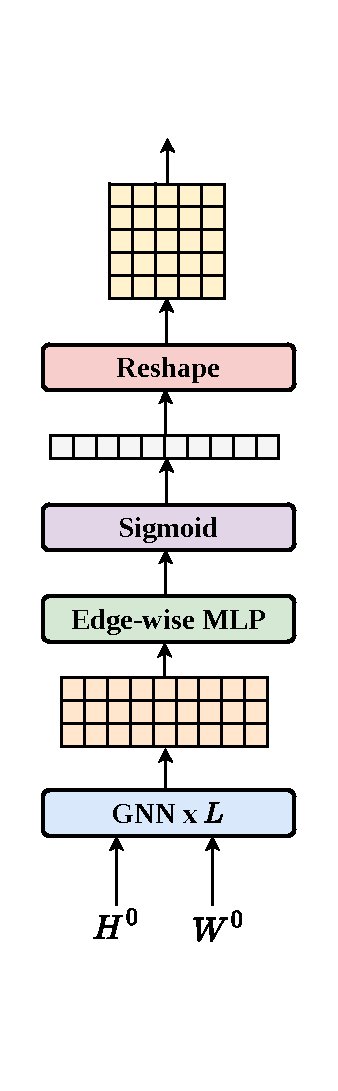
\includegraphics[height=0.34\textheight]{figures/gnn.pdf}%
    }
    \subfloat[Multi-trajectory guidance]{%
        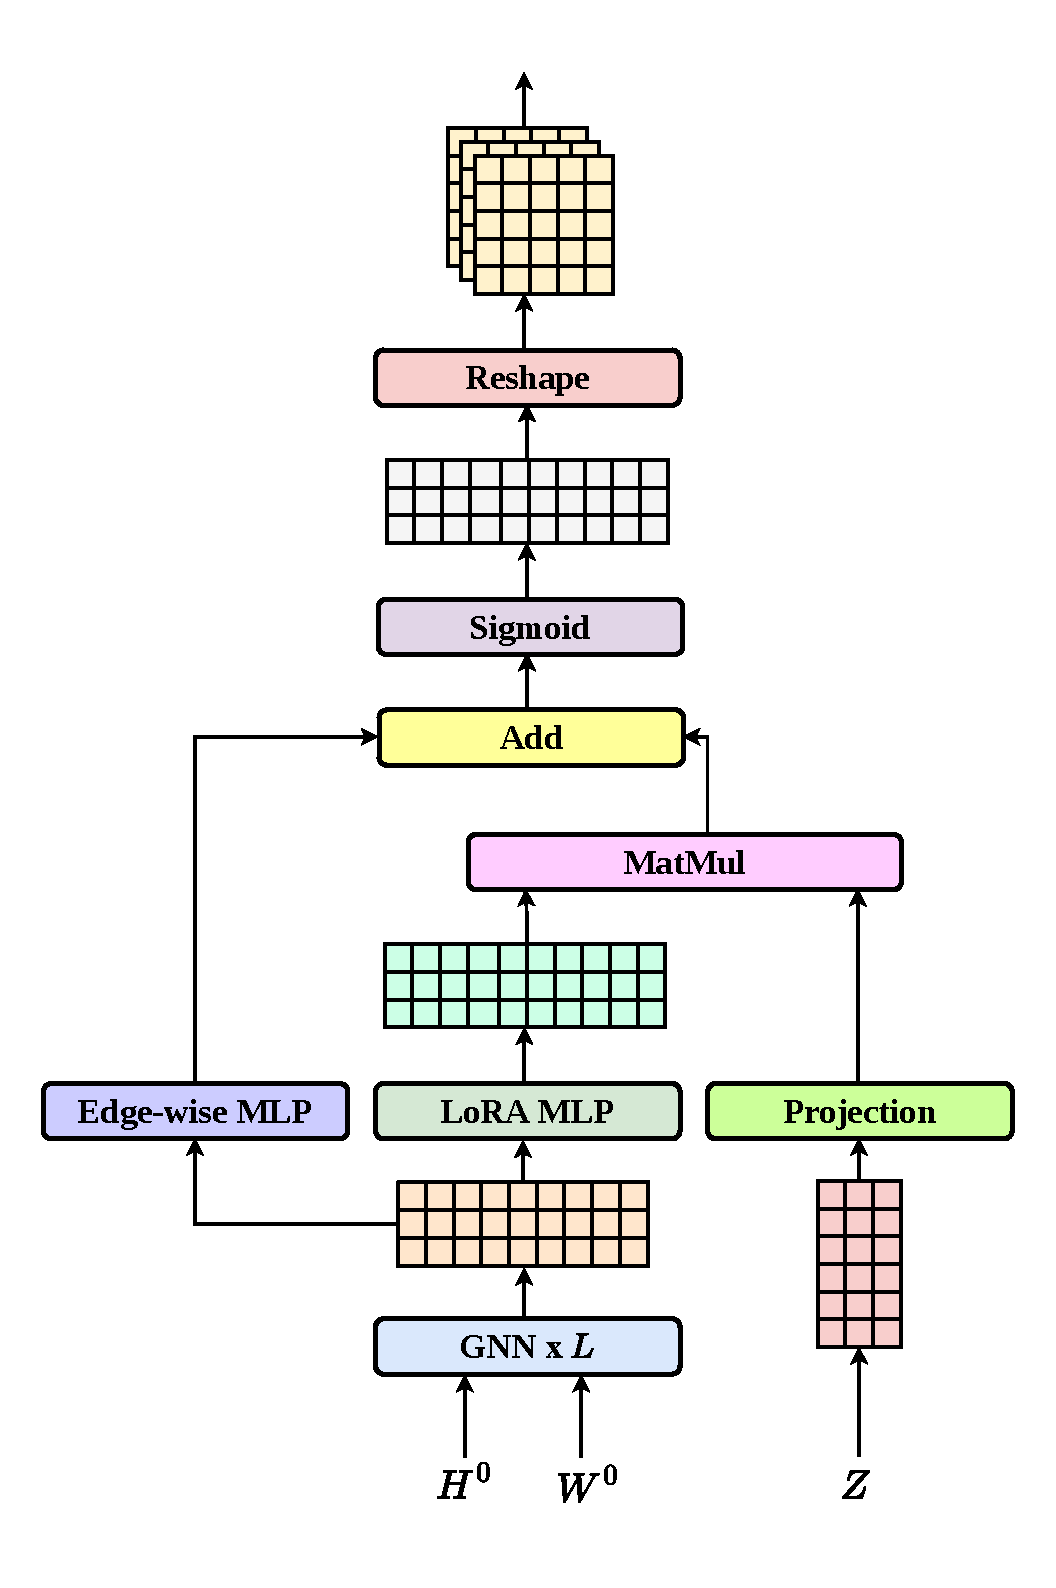
\includegraphics[height=0.34\textheight]{figures/moe.pdf}%
    }\hfill

\caption{Comparison between a single dynamic guidance field and trajectory-diverse guidance. The \DyNACO{} policy maps each macro-state to one sparse guidance field, whereas \DyNACS{} maps the same state to multiple guidance fields that steer disjoint ant groups within one shared search process.}
    \label{fig:multi-head-lora-gnn}
\end{figure}

\subsection{Mixture-Based Trajectory Guidance}
\label{sec:tdg-formulation}

We extend the semi-MDP in Section~\ref{sec:mdp} by augmenting dynamic guidance with a discrete behavior index. At macro-step $h$, the state remains
\begin{equation}
\mathcal{S}_h=(G,\tau^{(h,0)},b^{(h)}),
\end{equation}
but the policy action is now a set of $R$ behavior-conditioned guidance fields,
\begin{equation}
a_h = \{z_\theta^{(r)}(\mathcal{S}_h)\}_{r=1}^{R},
\qquad
z_\theta^{(r)}(\mathcal{S}_h)\in\mathbb{R}^{N\times K}.
\end{equation}
Each behavior $r$ defines a trajectory distribution for ants assigned to that behavior:
\begin{equation}
\log p_r^\theta(j \mid i; h, s)
= \alpha \log \tau^{(h,s)}_{ij}
+ \beta \log \eta_{ij}
+ \gamma z_{ij}^{(r)}(\mathcal{S}_h).
\label{eq:multi-trajectory-kernel}
\end{equation}
Thus, \DyNACS{} does not run $R$ independent solvers. It defines $R$ behavior-conditioned distributions over perturbation trajectories while preserving the same macro-state, incumbent solution, pheromone update, and SRR projection.

Let $\mathcal{A}_r^{(h,s)}$ be the ants assigned to behavior $r$ at inner iteration $s$. The transition cost for a macro-step is still measured over the combined population,
\begin{equation}
C_h =
\frac{1}{S m}\sum_{s=1}^{S}\sum_{r=1}^{R}
\sum_{a\in\mathcal{A}_r^{(h,s)}} C(\hat{\pi}_{a,s}),
\end{equation}
but each trajectory log-probability is evaluated under its assigned behavior,
\begin{equation}
\log \pi_\theta(\pi_{a,s}, r\mid\mathcal{S}_h)
= \log \omega_r^{(h)}
+ \sum_{t=1}^{T_a}\log p_r^\theta(v_t\mid u_t;h,s),
\end{equation}
where $\omega_r^{(h)}$ is the routing weight for behavior $r$. This formulation turns neural guidance from one homogeneous transition bias into a mixture of trajectory distributions: each behavior is evaluated through the quality of its refined trajectories, while all behaviors cooperate through the shared colony state.

\subsection{Behavior-Conditioned Guidance Generation}
\label{sec:tdg-policy}

The mixture model shares the state representation used by \DyNACO{} and learns multiple behavior-conditioned guidance maps on top of that representation. Let
\begin{equation}
\{e_{ij}^{(h)}\}_{(i,j)\in G}
=
\operatorname{GNN}_{\theta}
\bigl(G,\tau^{(h,0)},b^{(h)}\bigr)
\end{equation}
denote the sparse edge embeddings produced from the current macro-state. A shared guidance map $g_0$ captures common preferences over candidate edges, while $R$ behavior-conditioned residual maps $\{\Delta_r\}_{r=1}^{R}$ specialize this representation into distinct trajectory biases:
\begin{equation}
z_{ij}^{(r)}(\mathcal{S}_h)
= g_0(e_{ij}^{(h)}) + \Delta_r(e_{ij}^{(h)}),
\qquad r=1,\ldots,R,
\label{eq:multi-trajectory-logit}
\end{equation}
This parameterization makes the behavior-conditioned distributions comparable because they are grounded in the same encoded search state, while the residual maps let them express different edge-ordering preferences. In this sense, the mixture is not a collection of independent policies; it is a structured factorization of one state-aware policy into a shared search representation and multiple behavior-conditioned guidance maps.

We use a low-rank parameterization for the residual behavior maps to keep the mixture lightweight. In one equivalent form, the behavior-specific map is
\begin{equation}
W_r = W_0 + \frac{\alpha_{\mathrm{L}}}{d_{\mathrm{L}}}B_rA_r,
\end{equation}
where $W_0$ is shared, $A_r$ and $B_r$ are behavior-specific low-rank factors, and $d_{\mathrm{L}}$ is the adapter rank. Equivalently, the residual map can be written as
\begin{equation}
\Delta_r(e_{ij}^{(h)})
= \phi(e_{ij}^{(h)})^\top \psi_r + c_r,
\end{equation}
with an edge factor $\phi(\cdot)$ and a behavior code $\psi_r$. Both forms preserve the main computational property: the GNN is evaluated once per macro-state, and the mixture adds only lightweight behavior-specific maps. The resulting output is a sparse tensor in $\mathbb{R}^{R\times N\times K}$, matching the candidate graph used by the ACO backend.

\subsection{Shared Search Memory}
\label{sec:tdg-shared-colony}

At each inner ACO iteration, the ant population is partitioned into groups $\{\mathcal{A}_r\}_{r=1}^R$. Ants in group $r$ sample perturbation trajectories under $p_r^\theta$, but all groups start from the same reference solution and contribute to the same post-SRR candidate pool. The best refined trajectory among the combined population updates the incumbent, and the shared pheromone field is updated from that incumbent. The next macro-state therefore aggregates the effect of all behavior-conditioned distributions:
\begin{equation}
\mathcal{S}_{h+1}
=
\mathcal{T}_{\mathrm{ACO}}
\bigl(\mathcal{S}_h,\{z_\theta^{(r)}(\mathcal{S}_h)\}_{r=1}^{R}\bigr).
\end{equation}
This coupling is the key difference between trajectory-diverse guidance and independent multi-start search. Independent colonies would maintain separate pheromone fields and exchange information only through final solution selection. In \DyNACS{}, the behaviors interact through shared search memory at every inner iteration: a behavior that discovers a useful perturbation can reinforce the common colony state, while other behaviors can later exploit or counteract that reinforcement.

\subsection{Online Behavior Routing}
\label{sec:tdg-allocation}

The simplest trajectory-diverse variant routes ants uniformly across behaviors. We also use an online routing rule that shifts ant budget toward behaviors that have recently produced stronger refined trajectories. The rule keeps inference lightweight: it updates only running utilities and integer ant counts, without changing network parameters or maintaining separate solver states. Let $u_r^{(h)}$ denote the running utility for behavior $r$ at macro-step $h$, where larger values indicate better recent performance. Given the refined costs from ants assigned to behavior $r$, we form a per-step score
\begin{equation}
s_r^{(h)}
= -\operatorname{TopQMean}_{a\in\mathcal{A}_r}
\!\left[C(\hat{\pi}_{a,h})\right],
\label{eq:trajectory-prior-score}
\end{equation}
where the top-$Q$ mean reduces sensitivity to a single lucky ant and becomes the negative best cost when $Q=1$. Scores are normalized across behaviors and accumulated with an exponential moving average,
\begin{equation}
u_r^{(h+1)}
= (1-\mu)u_r^{(h)}+\mu\,\operatorname{Norm}(s_r^{(h)}).
\end{equation}
The next routing weights are
\begin{equation}
w_r^{(h+1)}
=
\frac{\exp(u_r^{(h+1)}/\lambda)}
{\sum_{r'=1}^{R}\exp(u_{r'}^{(h+1)}/\lambda)}.
\label{eq:trajectory-prior-weights}
\end{equation}
We then project $m w_r^{(h+1)}$ to integer ant counts $m_r^{(h+1)}$ with $\sum_r m_r^{(h+1)}=m$ and at least one ant for each active behavior. Uniform routing is recovered by fixing $w_r=1/R$. The rule changes only which behavior each ant follows; it does not create separate pheromone states or separate local-search procedures.

\subsection{Training and Inference}
\label{sec:tdg-training}

Training \DyNACS{} uses the same trajectory-aware PPO interface as \DyNACO{}, but conditions the trajectory likelihood on the assigned behavior. During training, the mixture acts as a strategy-discovery mechanism: all behaviors are evaluated through the shared colony, and the policy update is formed from the strongest behavior-conditioned trajectory group in that rollout. During inference, the learned behavior-conditioned maps are fixed and only the routing weights change online, allowing the search to adapt to the current instance without gradient updates. Let
\begin{equation}
r_h^\star = \operatorname*{arg\,max}_{r\in\{1,\ldots,R\}} s_r^{(h)}
\end{equation}
denote the behavior with the best refined trajectory score at macro-step $h$. For an ant assigned to this behavior, the PPO ratio is
\begin{equation}
\rho_{a,s}^{(r_h^\star)}(\theta)
=
\exp\!\left(
\bar{\ell}_{a,s}^{(r_h^\star)}(\theta)
-\bar{\ell}_{a,s}^{(r_h^\star)}(\theta_{\mathrm{old}})
\right),
\end{equation}
where $\bar{\ell}_{a,s}^{(r_h^\star)}$ is the per-decision normalized log-probability under $p_{r_h^\star}^\theta$. The clipped objective is applied to the selected behavior-conditioned trajectories:
\begin{multline}
\mathcal{L}_{\mathrm{TD}}(\theta)
= -\mathbb{E}_{a\in\mathcal{A}_{r_h^\star},s}\Big[
\min\big(
\rho_{a,s}^{(r_h^\star)}(\theta)\hat{A}_{a,s},\\
\operatorname{clip}(\rho_{a,s}^{(r_h^\star)}(\theta),1-\epsilon,1+\epsilon)
\hat{A}_{a,s}\big)\Big].
\end{multline}
The other behaviors are still part of the search transition because their refined trajectories can update the shared incumbent, pheromone field, and future routing utilities. Optionally, a small information-theoretic diversity regularizer can be applied to the mixture by maximizing the Jensen divergence among the row-wise transition distributions induced by $\{z^{(r)}\}_{r=1}^R$. This regularizer is not a separate solver objective; it only discourages all behaviors from collapsing to the same transition distribution.

\begin{algorithm}[t]
\caption{Trajectory-diverse guidance with online behavior routing for \DyNACS{}.}
\label{alg:trajectory-diverse}
\begin{algorithmic}[1]
\REQUIRE $\theta$ (shared encoder and behavior-conditioned maps), $R$ (behaviors), $m$ (ants), $H$ (outer steps), $S$ (inner steps)
\STATE Initialize $\tau^{(1,0)} \gets \tau_{\max}$, $b^{(1)} \gets \textsc{Greedy}(x)$, and routing utilities $\{u_r^{(1)}\}_{r=1}^R$
\FOR{$h = 1 \to H$}
    \STATE Encode $\mathcal{S}_h=(G,\tau^{(h,0)},b^{(h)})$
    \STATE Emit behavior-conditioned guidance fields $\{z_\theta^{(r)}(\mathcal{S}_h)\}_{r=1}^R$
    \STATE Route ants $\{m_r^{(h)}\}_{r=1}^R$ using uniform weights or Eqs.~\eqref{eq:trajectory-prior-score}--\eqref{eq:trajectory-prior-weights}
    \FOR{$s = 1 \to S$}
        \FOR{$r = 1 \to R$}
            \STATE Sample $m_r^{(h)}$ perturbation trajectories under $p_r^\theta(\cdot \mid \mathcal{S}_h,\tau^{(h,s)})$
        \ENDFOR
        \STATE Apply SRR to all sampled trajectories
        \STATE Update $b^{(h)}$ with the best refined trajectory from the combined population
        \STATE Update $\tau^{(h,s+1)}$ using the shared incumbent
        \STATE Update routing utilities $\{u_r\}_{r=1}^R$ from refined trajectory costs
    \ENDFOR
    \STATE $\tau^{(h+1,0)} \gets \tau^{(h,S)}$; \, $b^{(h+1)} \gets b^{(h)}$
\ENDFOR
\end{algorithmic}
\end{algorithm}


% ======================================================================
% 3.2 The Perturbative Environment
% ======================================================================
\section{Scalable Search Environment}
\label{sec:computational-alignment}
\label{sec:backend}

The previous two sections define what the policy observes and how one or several guidance fields shape search behavior. We now give the search environment through which those policy outputs affect the solver. This environment is shared by \DyNACO{} and \DyNACS{}: it converts edge-level guidance into short stochastic perturbation trajectories, then projects those trajectories back to locally consistent solutions before rewards are assigned. Its role is to keep the neural decision horizon short enough for policy learning while preserving the refinement quality expected from ACO\@. We realize this environment with two mechanisms: \emph{perturbative sampling}, which changes the action object from a full tour to a small set of edge interventions, and \emph{Scope-Restricted Refinement (SRR)}, which performs local projection around the affected region so that rewards remain causally tied to the sampled interventions.

\smallskip\noindent\textbf{Perturbative Sampling.}
In prior neural-guided ACO frameworks~\cite{deepaco,gfacs,gtgaco}, each ant constructs a tour from scratch. This makes the policy responsible for a sequence of $N$ edge decisions, which becomes expensive at large scales and exposes learning to sequential error accumulation. It also leaves no explicit reference state around which a post-processing step can preserve credit assignment. We instead use the current incumbent as a reference trajectory and let each ant modify only a small subset of candidate edges on a sparse $K$-nearest-neighbor graph. For \TSP{}, this perturbation interface follows~\cite{faco}; for \CVRP{}, we instantiate the same interface with capacity-aware feasibility checks (Appendix~\ref{app:backend}).

At sampling iteration $s$ of guidance update $h$, transition probabilities combine pheromones, heuristics, and neural guidance via a \emph{guidance weight} $\gamma$:
\begin{equation}
\log p^\theta(j \mid i; h, s) = \alpha \log \tau^{(h,s)}_{ij} + \beta \log \eta_{ij} + \gamma\, z_{ij}(\mathcal{S}_h).
\label{eq:held-logits}
\end{equation}
During training $\gamma{=}1$ (constant forcing); at inference $\gamma$ may be annealed (see Section~\ref{sec:inference}). The policy outputs $z_\theta(\mathcal{S}_h)$ once per guidance update and holds it constant for $S$ sampling iterations, decoupling neural guidance (updated at guidance-update boundaries) from pheromone dynamics (updated at every sampling iteration). Crucially, prior neural-ACO methods~\cite{deepaco,gfacs,gtgaco} replace the heuristic term~$\eta_{ij}$ with neural output, discarding hand-crafted domain knowledge. We instead retain both $\tau_{ij}$ and $\eta_{ij}$, and introduce neural logits~$z_{ij}$ as a third, additive term in Eq.~\eqref{eq:held-logits}. This preserves the domain knowledge encoded in $\eta$ while letting the network provide complementary, state-dependent guidance.

Formally, each ant initializes from the incumbent solution $b^{(h)}$ and executes up to $M$ stochastic edge interventions. At each intervention, the ant samples a successor node $v$ from the feasible candidate set according to Eq.~\eqref{eq:held-logits}; edges $(u,v)$ absent from the incumbent are recorded as anchors for the subsequent scope-restricted refinement mechanism. The trajectory log-probability decomposes over stochastic decisions:
\begin{equation}
\log \pi_\theta(\pi_{a,s} \mid \mathcal{S}_h) = \sum_{t=1}^{T_a} \log p^\theta(v_t \mid u_t; h, s),
\label{eq:logp-trajectory}
\end{equation}
where $T_a \le M$ denotes the number of stochastic interventions, i.e., steps at which multiple candidates were feasible. This formulation changes the learning problem from constructing all $N$ tour edges to selecting a small intervention set of size at most $M \ll N$. Consequently, the decision horizon is bounded by $M$ rather than $N$, preventing the error accumulation inherent in $\mathcal{O}(N)$-length sequential construction and stabilizing policy learning at scale. The localized intervention set also defines the region on which refinement should be allowed to affect the reward.

\smallskip\noindent\textbf{Scope-Restricted Refinement.}
\label{sec:localized-ls}
In neural-guided ACO~\cite{deepaco,gfacs,gtgaco}, refinement is part of the training environment: the post-refinement cost is the reward signal used for policy-gradient updates. This creates a projection-credit trade-off. If refinement is too weak, sampled trajectories remain under-refined and rewards are noisy. If refinement is too strong and unconstrained, it can rewrite most of the sampled intervention, so the final cost reflects the refinement heuristic rather than the neural decision. We refer to this failure mode as \emph{gradient washout}.

Figure~\ref{fig:credit_assignment} illustrates this trade-off using DeepACO on TSP-200 under three refinement strategies. With \emph{Full 2-opt} (red), the policy fails to converge because the local search heavily rewrites the sampled tour and severs the causal link between actions and rewards. \emph{Limited 2-opt} (orange) preserves more of the learning signal by stopping after $N/4$ swaps, but this early stopping bottlenecks solution quality. \emph{Neural Local Search}~\cite{deepaco} (blue) improves quality by using the neural policy to score candidate swaps, but it is not scalable because it requires neural evaluations inside the refinement loop.

\begin{figure}[t]
    \centering
    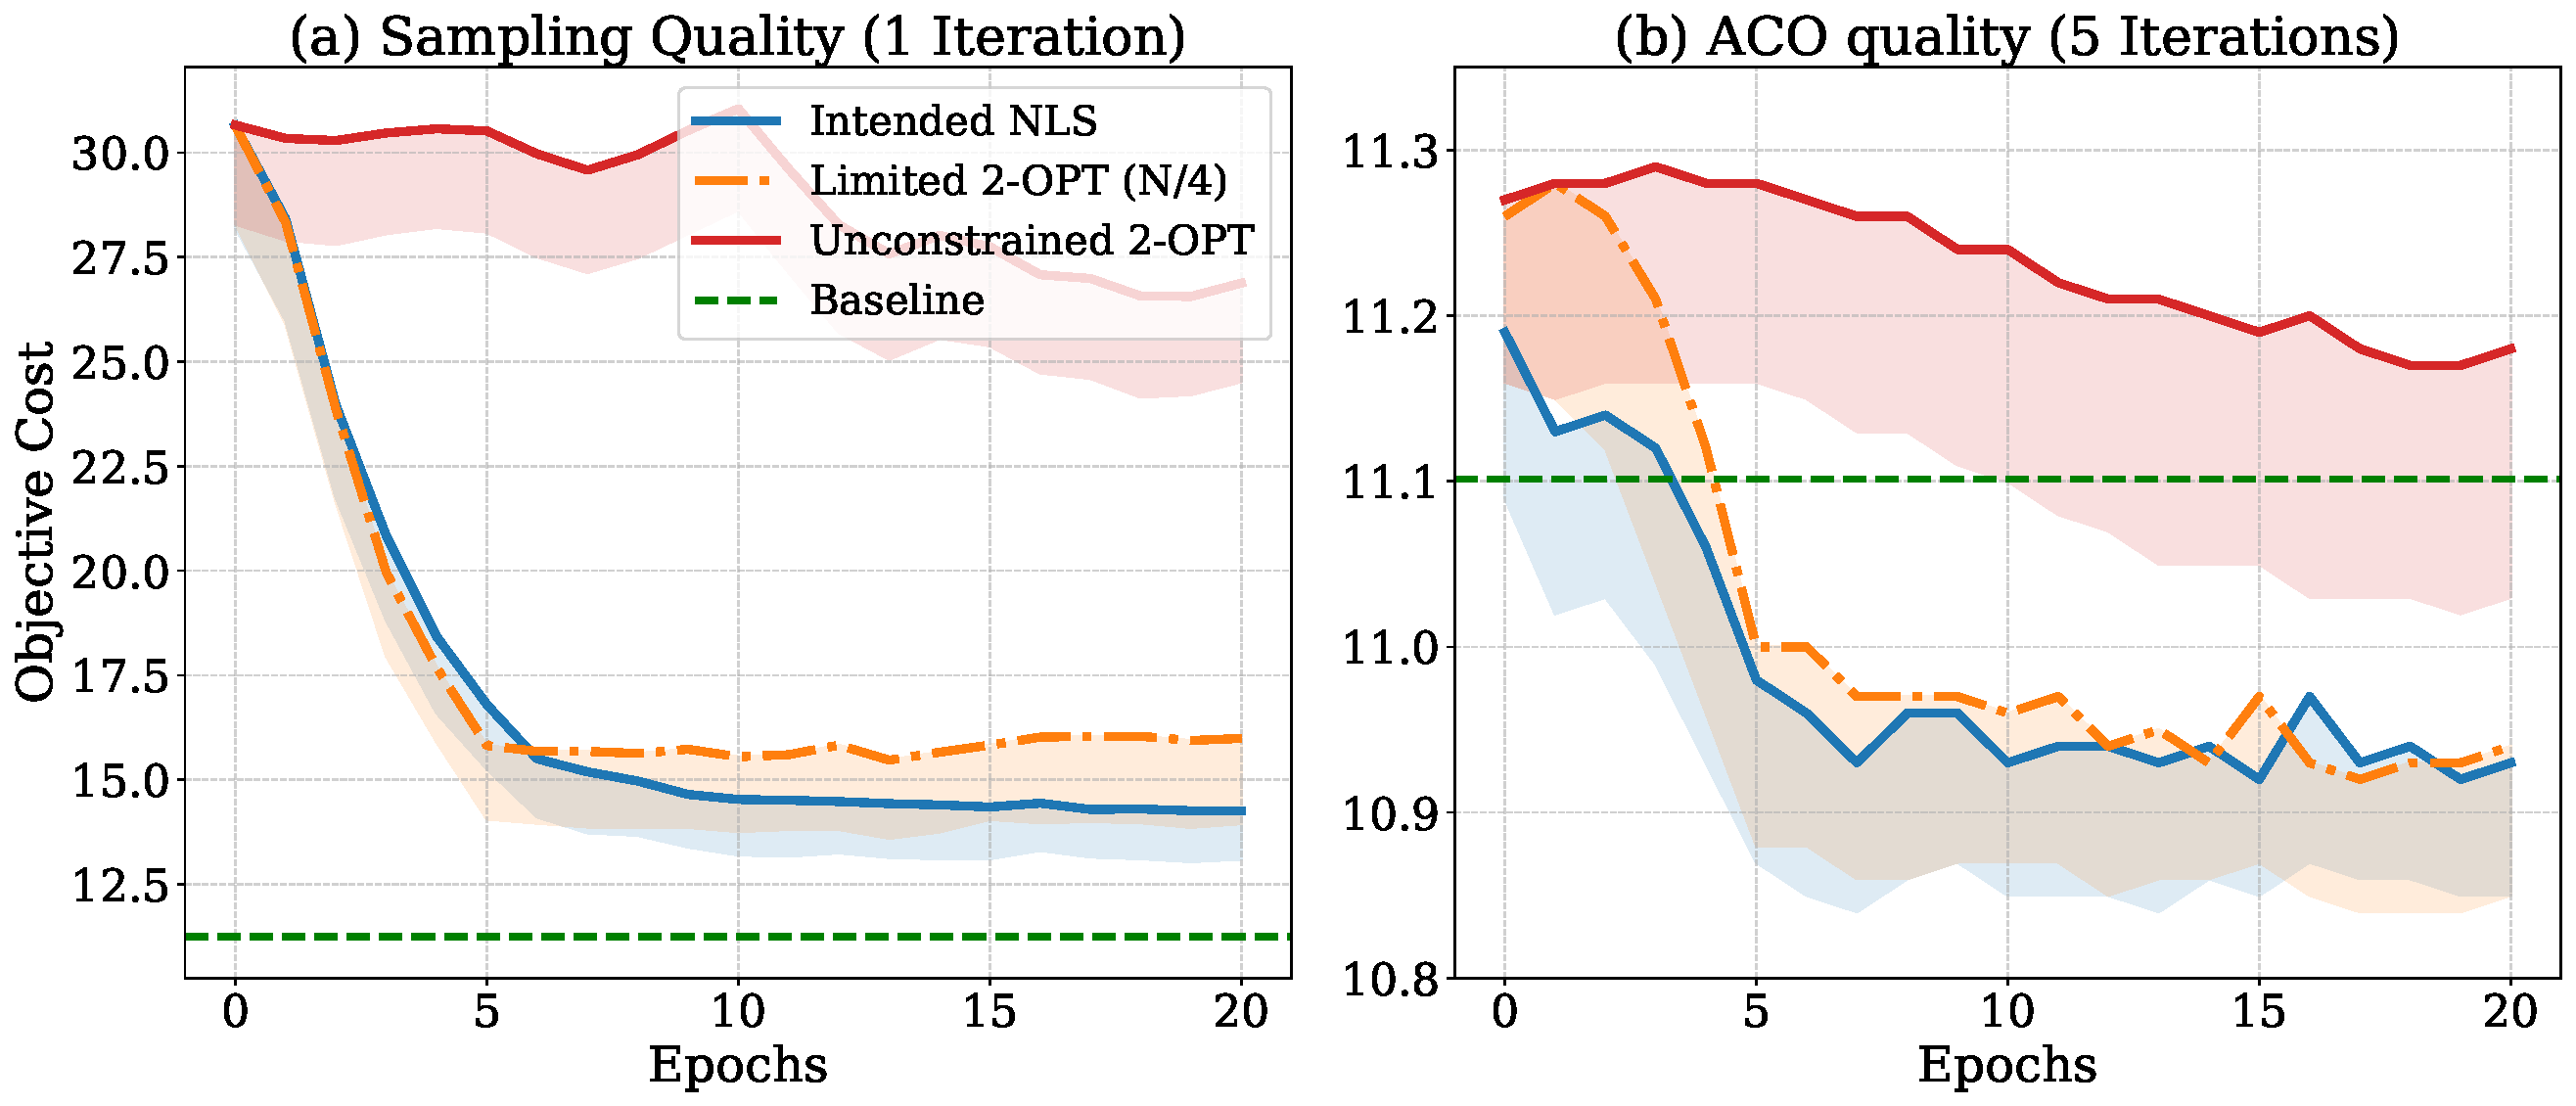
\includegraphics[width=\columnwidth]{figures/nls_vs_limited_vs_unconstrained.pdf}
    \caption{Credit-assignment trade-off under different local-search strategies when training DeepACO on TSP-200.}
    \label{fig:credit_assignment}
\end{figure}

Scalability imposes an additional constraint. Standard 2-opt costs $\mathcal{O}(N^2)$ per tour, which is prohibitive when refinement must be applied to every ant at every iteration. Classical large-scale ACO methods~\cite{partialACO, P-ACO} reduce this cost by applying local search only occasionally or only to elite ants. This is unsuitable for policy-gradient training, where per-ant advantages require post-refinement costs for all sampled ants. Thus, the refinement operator must satisfy three requirements simultaneously: it must preserve the causal link between policy actions and rewards, refine tours to convergence rather than stop at an arbitrary budget, and have cost independent of the full instance size.

We satisfy these requirements using Scope-Restricted Refinement (SRR), inspired by~\cite{faco}. The key observation is that perturbation-based ants start from an incumbent solution that is already locally optimized under the candidate graph. Since an ant modifies only a small set of edges, any newly introduced sub-optimality is localized around those interventions. SRR therefore acts as a local projection operator: it initializes a checklist with the endpoints of the perturbed edges and repeatedly applies improving candidate-graph refinement moves involving checked nodes, reactivating affected neighbors after each accepted move. In routing, these refinement moves are instantiated with candidate-limited 2-opt for \TSP{} and capacity-preserving relocate/swap/2-opt* operators for \CVRP{}; Appendix~\ref{app:setup} gives the algorithmic details. Conceptually, SRR propagates repair outward from the intervention region until no improving move remains within its scope.

Specifically, SRR provides the three properties required for training. First, because refinement is restricted to the neighborhood of the policy's perturbations, the post-refinement cost remains causally tied to the sampled actions, preserving credit assignment. Second, unlike truncated local search, SRR runs to convergence within its scope; assuming the incumbent was already candidate-graph 2-opt optimal, this restores candidate-graph 2-opt optimality after the perturbation. Third, the refinement cost scales with the perturbation size, $\mathcal{O}(M \cdot K)$, rather than the instance size, $\mathcal{O}(N^2)$, allowing SRR to be applied to every ant at every iteration even at $N{=}100$K.

% \smallskip\noindent\textbf{Scope-Restricted Refinement.}
% \label{sec:localized-ls} Other than the scalability, integrating local search (LS) into policy-gradient training presents another challenge: \emph{gradient washout}. If a powerful LS drastically rewrites the entire tour, it severs the causal link between the policy's initial decisions and the final rewards, destroying the learning signal. Figure~\ref{fig:credit_assignment} tracks the training progression of DeepACO on TSP-200 under three distinct LS strategies. When employing an \emph{Unconstrained 2-OPT} (red curve), the policy completely fails to converge. Because the unrestricted heuristic heavily rewrites the ant's initial tour, the causal link is thus severed. DeepACO attempts to mitigate this via \emph{Limited 2-OPT ($N/4$)} (orange curve); this restores the gradient signal but bottlenecks solution quality due to early stopping. Alternatively, its \emph{Intended NLS} (blue curve) achieves the lowest cost by using the neural policy to evaluate every candidate swap; however, this severely limits scalability by requiring $\mathcal{O}(N \cdot K)$ neural forward passes inside the refinement loop.
% The computational burden is exacerbated at scale: standard 2-opt costs $O(N^2)$ per tour, prohibitive for every ant on every iteration at $N{=}100$K. Classical large-scale ACO~\cite{partialACO, P-ACO} mitigates this by applying LS \emph{sparingly} (every few iterations) and \emph{elitely} (only to the best or top-$k$ ants), but policy-gradient training is incompatible: per-ant advantages require post-LS costs for \emph{every} ant at \emph{every} iteration. Capping swaps at a fixed budget reduces cost at the expense of quality, and the cap still scales with $N$ rather than the perturbation size.

% \begin{figure}[t]
%     \centering
%     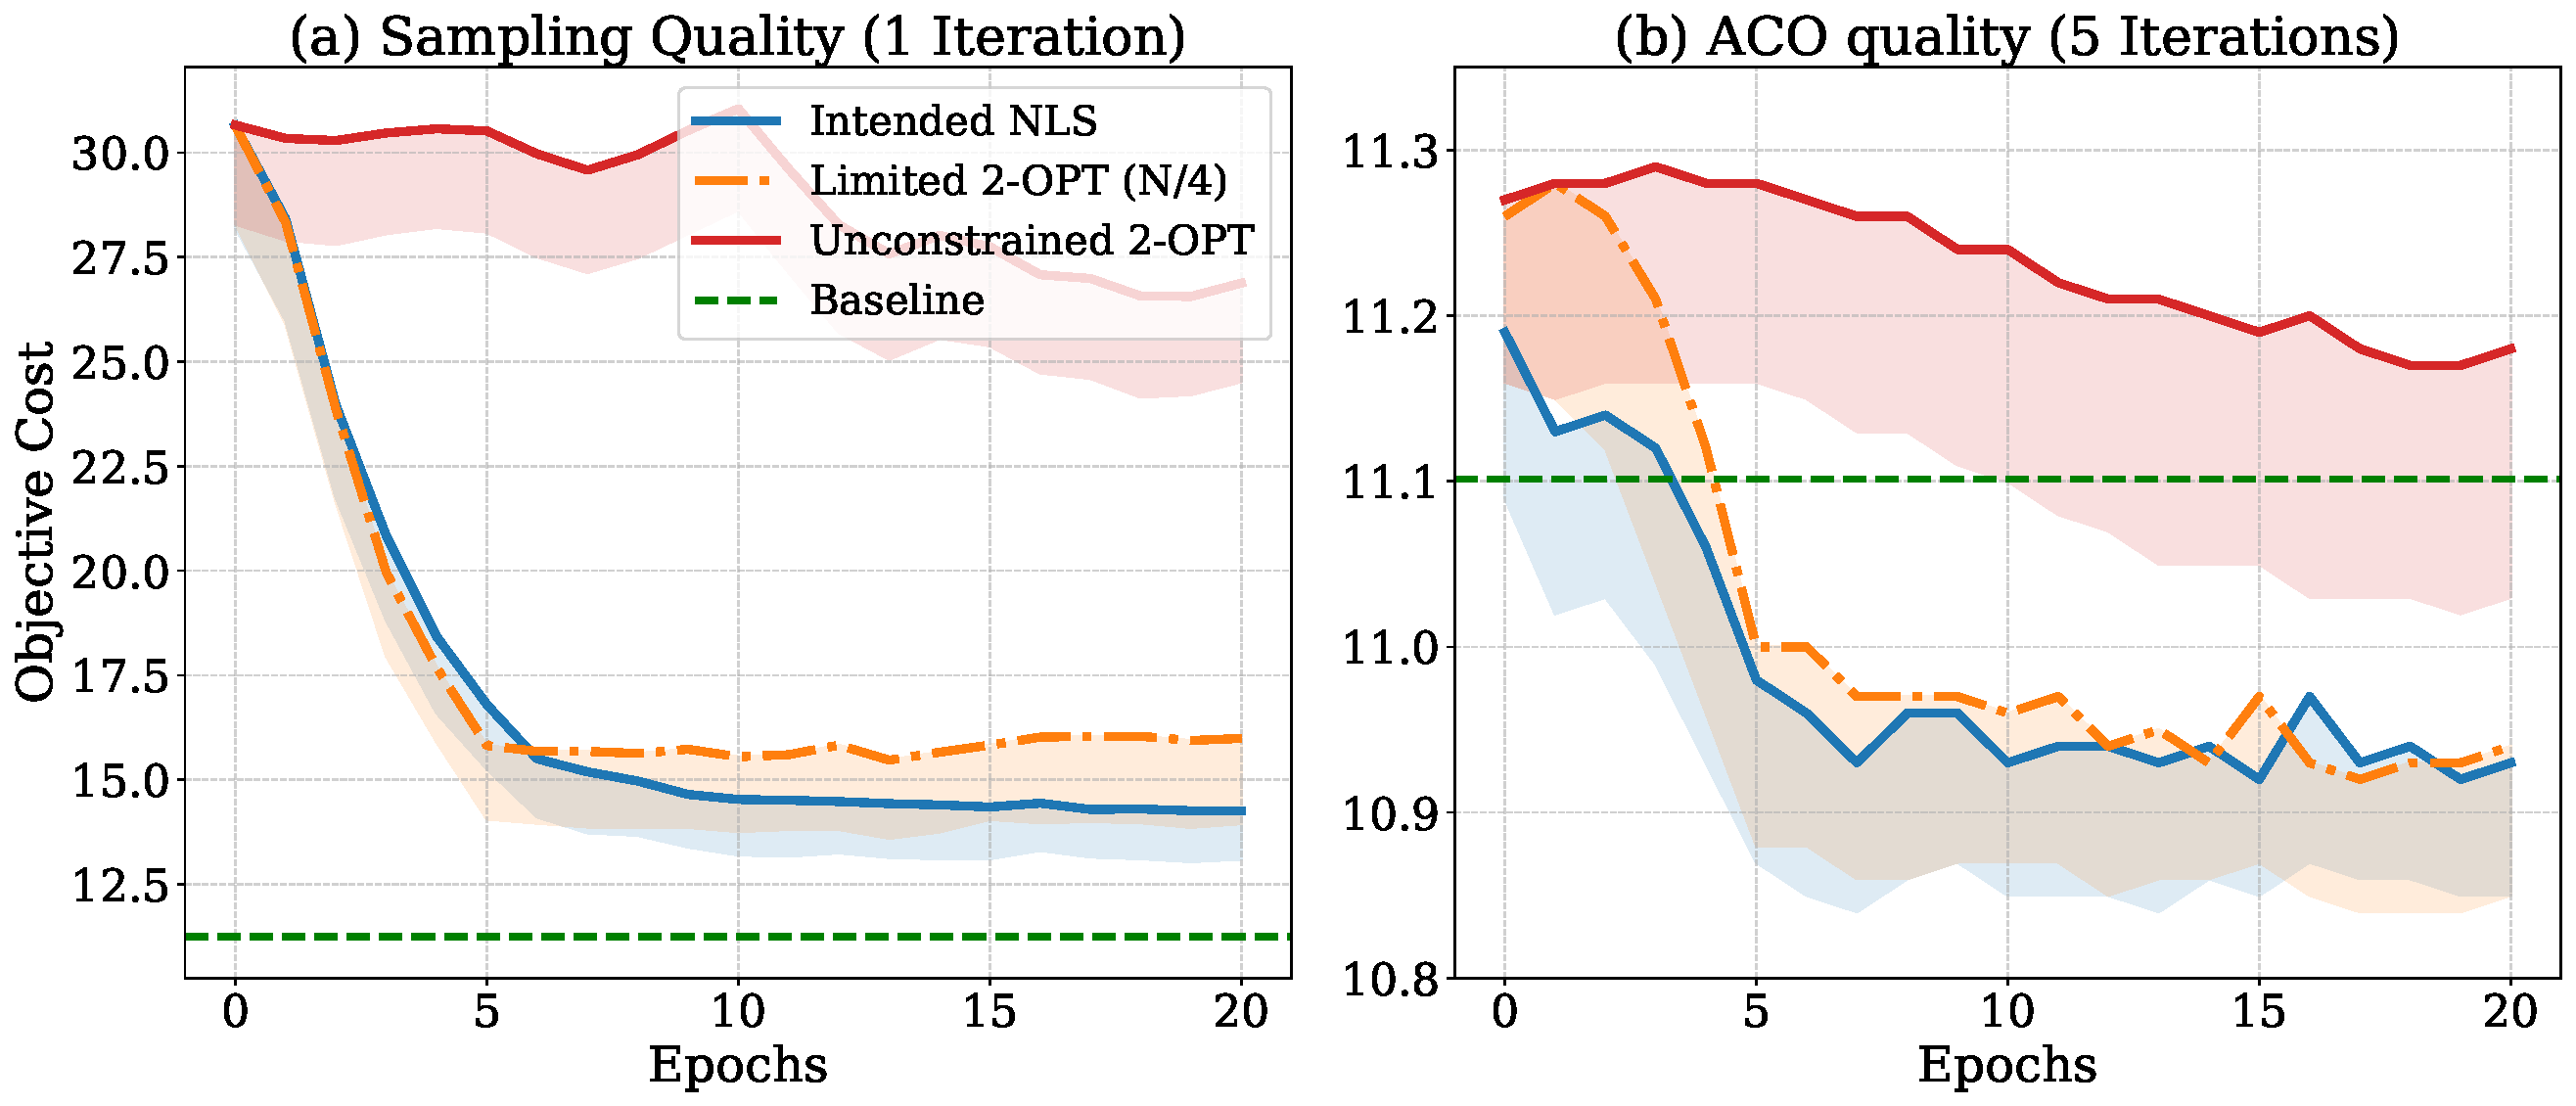
\includegraphics[width=\columnwidth]{figures/nls_vs_limited_vs_unconstrained.pdf}
%     \caption{The gradient washout trade-off: three LS strategies for training DeepACO on TSP-200.}
%     \label{fig:credit_assignment}
% \end{figure}

% We resolve this dilemma using Scope-Restricted Refinement (SRR)~\cite{faco}. The key insight is that the incumbent solution is generally already locally optimal.
% When an ant perturbs this solution, it creates a localized region of sub-optimality.
% SRR operates as a targeted repair mechanism, conceptually similar to a Breadth-First Search (BFS), that propagates improvements outward from the perturbed edges only.
% Unlike DeepACO's truncation strategy, SRR runs to convergence within its scope.
% Because the unperturbed regions of the tour were already optimized under the candidate graph, repairing the perturbed region restores 2-opt optimality with respect to the candidate-graph move set. SRR simultaneously provides three properties that existing designs achieve only in isolation:
% \begin{enumerate}
%     \item \emph{Stable Credit Assignment}: confining refinement to the neighborhood of the policy's actions preserves the causal link between neural decisions and rewards, matching NLS's credit-assignment role without additional neural forward passes.
%     \item \emph{Within-Scope Convergence}: unlike truncated LS, SRR runs to convergence, yielding a tour that is 2-opt optimal on the candidate-graph move set within the perturbed region.
%     \item \emph{Size-Independent Scalability}: refinement cost scales as $O(M{\cdot}K)$ with the perturbation size, not $O(N^2)$ with instance size, so SRR can be applied to \emph{every} ant at \emph{every} iteration (a requirement for policy-gradient training) even at $N{=}100$K.
% \end{enumerate}
% SRR thus combines the efficiency of truncated LS with the credit-assignment benefit of NLS: by guaranteeing that unperturbed regions remain locally optimal, convergent refinement within the perturbation scope is both sufficient and inexpensive (formal optimality argument in Section~\ref{app:credit}).

\smallskip\noindent\textbf{Stabilized Pheromone Dynamics.}
\label{sec:smoothed-mmas}
\MMAS{}~\cite{maxmin} bounds pheromones to $[\tau_{\min}, \tau_{\max}]$ to prevent premature convergence, but couples these bounds to solution cost, creating non-stationary input distributions for the state-aware policy. We instead adopt fixed bounds ($\tau_{\max}{=}1$, $\tau_{\min}{=}1/K$) and update via convex interpolation:
\begin{equation}
\tau^{(h,s+1)}_{ij} \leftarrow (1-\rho)\tau^{(h,s)}_{ij} + \rho \cdot \mathcal{T}_{ij},
\label{eq:smoothed-mmas}
\end{equation}
where $\mathcal{T}_{ij} = \tau_{\max}$ if $(i,j)$ is in the best solution, else $\tau_{\min}$.
This yields scale-invariant state representations and stabilizes training.
While this simplification may reduce the solution quality of the \emph{unguided} solver compared to highly tuned \MMAS{} dynamics, our ablations (Section~\ref{sec:ablations}) show that \DyNACO{} with stabilized bounds outperforms both (i)~unguided ACO with standard \MMAS{} updates and (ii)~neural-guided ACO retaining the original update rule.

\subsection{Inference Controls}
\label{sec:inference}
We use constant guidance ($\gamma{=}1$) during training, with no annealing or phased scheduling.
At inference, the guidance weight~$\gamma$ (Eq.~\ref{eq:held-logits}) can be modulated via two strategies: \emph{guidance annealing}, which linearly decays $\gamma \to 0$ across inner iterations; and \emph{phased injection}, which withholds neural guidance for the first fraction of outer steps.
The specific configuration varies by problem and scale: for TSP, we apply annealing at all scales and additionally enable phased injection at TSP-1K; for CVRP, we apply phased injection only at longer iteration budgets ($I{\geq}5000$) and never anneal.

\subsection{Cost and Memory Scaling}
\label{sec:complexity}

The computational cost separates into sparse neural inference and ACO operations based on perturbations. The GNN encoder runs once per outer step on the $K$-NN graph, giving $\mathcal{O}(H L n K d)$ neural cost for $H$ guidance updates, $L$ layers, $n$ nodes, $K$ candidates, and hidden dimension $d$. During the ACO search, each of the $m$ ants performs at most $M$ stochastic interventions, and SRR scans only the affected candidate neighborhoods. Over $T=H S$ inner iterations, this gives $\mathcal{O}(T m M K)$ sampling and local projection cost.

The learned state and replay buffers are also sparse. Pheromone snapshots, edge features, feasible masks, and action traces are stored on the candidate graph, requiring $\mathcal{O}(nK)$ memory rather than $\mathcal{O}(n^2)$ dense heatmaps. The extension from \DyNACO{} to \DyNACS{} reuses the same encoder and adds only lightweight behavior maps. This cost profile is what allows neural guidance to remain active during large search runs instead of being used only as an initialization heuristic.
